% This stuff goes in a separate file because it'll change frequently
\newcommand{\draftfinal}{%
  %draft%
  final%
}

\includeonly{ % comment out lines so as to speed up compilation when working on specific chapter(s):
    titleE,
    titleL,
    %titleP,
    declaration,
    acknowledge,
    %publications,
    nomenclature,
    %summary,
    %introduction,
    %junctions,
    tlsmodel,
  %  startappendices
    }

%%%%%%%%%%%
%% PAPER TYPE
\newcommand{\paperoptions}{a4paper}

%%%%%%%%%%%
%% VERSIONS
%% Screen version(default): one+halfspaced, dropped caps, coloured hyperlinks, onesided

%To print on larger stock, uncomment this
%\renewcommand{\paperoptions}{b4paper}
 % separate file cos it's gonna change frequently
\documentclass[fleqn,USenglish,\classoptions,\draftfinal]{book}
\usepackage{ifdraft}

\usepackage{mathtools}    % amsmath equation env has funny spacing with hyperref :-( so...
\let\equation\gather \let\endequation\endgather
\usepackage{amssymb} 
\usepackage{dsfont}
\usepackage{mathspec}
%\usepackage{fontspec} %There are options I'll need for ligatures etc.. Read the doc.
\setromanfont[Ligatures={TeX, Common}, Numbers=OldStyle]{Skolar PE}
%\setmainfont[RawFeature={+ss02,+cv01,+ss05,+dlig},ItalicFeatures={RawFeature=+cv04,CharacterVariant=5:2}]{EB Garamond} %Good for old school s
\setsansfont{Idealist Sans}
\setmonofont{PragmataPro}
%\defaultfontfeatures{ Scale = MatchLowercase }

\setmathsfont(Digits,Latin,Greek)[Numbers={Lining,Proportional}]{Minion Pro}

\usepackage{ragged2e}  % load early, so things pick it up. [newcommands] to replace old ver

\usepackage{xunicode} %Extra unicode options for xetex
\usepackage{babel}
\usepackage{eqparbox}
\usepackage[rgb]{xcolor}
\usepackage[mode=buildmissing]{standalone} %TODO: buildnew doesn't work for xelatex. Find out what to do with this.
\usepackage{tikz}
\usepackage{pgfplots}
\pgfplotsset{compat=1.10}
\usetikzlibrary{shapes,arrows}
%\usepackage[final]{graphicx}
\usepackage{url}
\urlstyle{rm} 
\usepackage[sort&compress,mcite]{natbib}
\usepackage{bibentry} % for permissions
%choose cite formatting:
\renewcommand*{\citenumfont}[1]{\addfontfeature{Numbers=Lining}{#1}} % oldstyle looks wrong to me in brackets. TODO: This isn't fixing the issue
\citestyle{plain}           % numbers in square brackets
%\citestyle{nature}         % superscript.
%choose a number formatting for the biblist:
\renewcommand*{\bibnumfmt}[1]{\eqparbox[t]{bblnm}{\hfill#1.}}
\usepackage{bibunitsLSB}    % a problematic package. maybe matters whether before/after natbib?

% Thesis-specific formatting
\ifdblspc\usepackage{setspace} % before geometry, so that heightrounded works right.
\else
\newenvironment{singlespace}{}{}
\newenvironment{singlespace*}{}{}
\fi
\usepackage[\geomoptions]{geometry} % showframe?
\usepackage{tocbibind} % put things in the table of contents.

\usepackage{emptypage} % no page numbers or headers on empty pages

%%%%%%%%%%%%%%%%%%%%%%%%%%%%%%
%% FORMATTING
% I have lots of big figures, so allow pages with only a few lines of text
\renewcommand{\topfraction}{0.9}
\renewcommand{\bottomfraction}{0.6}
\setcounter{topnumber}{2}
\setcounter{bottomnumber}{2}
\setcounter{totalnumber}{2}
\renewcommand{\textfraction}{0.07}
\renewcommand{\floatpagefraction}{0.7}
\renewcommand{\dblfloatpagefraction}{0.7}
% flushbottom is in principle better than raggedbottom for twoside, but my life is too short to try to make this kind of document (lots of figures, section headings, equations) layout properly in LaTeX with flushbottom. the stretchy topskip is a trick to get (slightly) better pagebreaks:
\widowpenalty=10000 \raggedbottom  \addtolength{\topskip}{0pt plus 10pt}
\usepackage{fnbreak}% warn about footnotes broken across pages, or:
%\interfootnotelinepenalty=10000 % ...prevent split footnotes completely
\usepackage{sectsty} % load before fncychap
\sectionfont{\fontspec{Idealist Sans}\fontsize{15}{17}\selectfont}
\subsectionfont{\fontspec{Idealist Sans}\fontsize{13}{15}\selectfont}
%\sectionfont{\fontfamily{phv}\fontseries{m}\fontsize{15}{17}\selectfont}
%\subsectionfont{\fontfamily{phv}\fontseries{m}\fontsize{13}{15}\selectfont}
\usepackage[Sonny]{fncychap} % TODO: Change this
    \ChNameVar{\Large\fontspec{Idealist Sans}\selectfont}
    \ChTitleVar{\Large\fontspec{Idealist Sans}\selectfont}
    %\ChNameVar{\Large\fontfamily{phv}\selectfont}
    %\ChTitleVar{\Large\fontfamily{phv}\selectfont}
\usepackage{emptypage} % no page numbers or headers on empty pages
\usepackage[font={small},labelfont={bf},margin=15pt]{caption} % load after babel. also replaces hypcap.
\usepackage{threeparttable}
\usepackage{booktabs}
%\usepackage{csquotes}
\usepackage{textcase}
\usepackage{fancyhdr}
\DeclareRobustCommand*{\sclspaced}[1]{\addfontfeature{LetterSpace=20.0,Numbers=Lining}{\MakeTextLowercase{#1}}} \DeclareRobustCommand*{\scuspaced}[1]{\addfontfeature{LetterSpace=20.0,Letters= SmallCaps,Numbers=Lining}{#1}}
\fancyhf{}
\setlength{\unitlength}{22mm}
\newcommand{\doblob}{\rule[-.1\unitlength]{2\unitlength}{.5\unitlength}}
\newcommand{\rblob}{%
    \begin{picture}(0,0)
        \put(1.05,-\value{thumbcount}){\blob}
    \end{picture}}
\newcommand\lblob{%
    \begin{picture}(0,0)
        \put(-3.05,-\value{thumbcount}){\blob}
    \end{picture}
}
\newcounter{thumbcount}
\makeatletter
\newcommand\overview{}
\newcommand*{\listofthumbs}{%
    \cleardoublepage
    \thispagestyle{overview}%
    \@starttoc{thb}
    \mbox{}\newpage}
\makeatother
\newcommand*{\thumbwrite}[2]{\addtocontents{thb}{\string\thumbitem{#1}{#2}}}
\newcommand*{\thumbitem}[2]{\expandafter\gdef\expandafter\overview\expandafter{\overview
    \begin{picture}(0,0)
        \put(0.75,-#2){\llap{\Large{#1}}}
        \put(1.05,-#2){\doblob}
    \end{picture}}}
\newcommand*{\thumb}[1]{%
    \let\blob=\doblob
    \stepcounter{thumbcount}%
    \thumbwrite{#1}{\arabic{thumbcount}}}
\newcommand*{\nothumb}{\let\blob=\relax}
\nothumb
\newcounter{lframe}
\newcounter{rframe}
\pagestyle{fancy} % use the fancy header
\headfoot
%%%    %\pagestyle{headings} % use ordinary header
% Chapter headings in the list of figures:
\newcommand{\lofchap}[1]{%
    \addtocontents{lof}{\protect\addvspace{-10pt}}% Undo the unconditional 10pt skip from latex
    \addcontentsline{lof}{lofchapter}{\protect\numberline{\thechapter}#1}%
}

%%%%%%%%%%%%%%%%%%%%%%%%%%%%%%%
%% VERSIONING/CHANGE TRACKING
\usepackage[shadow,obeyDraft,colorinlistoftodos,textsize=small]{todonotes}
\usepackage{fixme}
\newcommand*\timFXtodo[3]{\todo[caption={#2}]{\begin{singlespace}#2\end{singlespace}}}
\FXRegisterLayout*[marginclue,marginnote,margin]{todo}{\timFXtodo}
\fxsetup{todo}
%\newcommand{\FXUser}[2]{\todo[caption={#2}]{\begin{singlespace}#2\end{singlespace}}}
\newcommand*{\xxx}[1]{\fxnote{#1}}
\newcommand*{\fixmelist}{\listoffixmes} % or listoftodos (nice color, missing figures)
\usepackage[markifdraft]{gitinfo2}

\ifdraft{%
%\usepackage{ocg}
%\newcommand*{\showkeyslabelformat}[1]{%
%    \begin{ocg}{labels}{lab}{1}\fbox{\normalfont\small\ttfamily#1}\end{ocg}}
\usepackage[color,notref,notcite]{showkeys} % notref for cleverref compat
%\makeatletter
%\def\SK@@ref#1>#2\SK@{%
%    \leavevmode\vbox to\z@{%
%        \begin{ocg}{references}{refs}{0}%
%        \vss
%        \SK@refcolor
%        \rlap{\vrule\raise .75em%
%            \hbox{\underbar{\normalfont\footnotesize\ttfamily#2}}}%
%        \end{ocg}}}%
%\makeatother
}{} % ifdraft

%%%%%%%%%%%%%%%%%%%%%%
%% MICROTYPOGRAPHY
\usepackage[babel,final]{microtype}

%%%%%%%%%%%%%%%%%%%%%%%%%%%%%%%%%
%% HYPERLINKS/PDF
%% these packages must come last:

%\PassOptionsToPackage{final,\hyperoptions,hyperfootnotes=false,linktoc=all,pagebackref}{hyperref}
\usepackage[final,\hyperoptions,hyperfootnotes=false,linktoc=all,pagebackref]{hyperref}
\usepackage{backref}

%\usepackage[a-1b]{pdfxLSB} % some bugs fixed/worked around by LSB. don't forget to update
\let\oldphantomsection\phantomsection
% Set up back references:
    \backrefparscanfalse
    \newcommand{\backrefnotcitedstring}{\relax}%(Not cited.)
    \newcommand{\backrefcitedsinglestring}[1]{Cited on page~#1.}
    \newcommand{\backrefcitedmultistring} [1]{Cited on pages~#1.}
    \AtBeginDocument{% to override babel
        \renewcommand{\backreftwosep}{~\&~}    % seperate 2 pages
        \renewcommand{\backreflastsep}{~\&~}} % seperate last of longer list
    \renewcommand*{\backref}[1]{}  % Disable standard
    \renewcommand*{\backrefalt}[4]{% Detailed backref
      \ifcase #1\backrefnotcitedstring%
      \or\backrefcitedsinglestring{#2}%
      \else\backrefcitedmultistring{#2}%
      \fi}

\usepackage[english]{cleveref} % after hyperref
\crefname{equation}{}{equations}
\crefname{figure}{figure}{figures}
\crefformat{equation}{(#2#1#3)}
\Crefformat{equation}{Equation~(#2#1#3)}
\crefformat{appendix}{#2appendix~#1#3}
\Crefformat{appendix}{#2Appendix~#1#3}
\crefformat{chapter}{#2chapter~#1#3}
\Crefformat{chapter}{#2Chapter~#1#3}
\crefformat{section}{#2section~#1#3}
\Crefformat{section}{#2Section~#1#3}
\crefformat{figure}{#2figure~#1#3}
\Crefformat{figure}{#2Figure~#1#3}
\crefformat{table}{#2table~#1#3}
\Crefformat{table}{#2Table~#1#3}


% controversial: cancel resetting page numbers at end of \frontmatter, for easier pdf navigation:
\makeatletter
\def\pagenumbering#1{\gdef\thepage{\csname @#1\endcsname \c@page}}
\makeatother

\newcommand*{\ie}{\textit{i.e.\ }}
\newcommand*{\etc}{\textit{etc.}}
\newcommand*{\eg}{\textit{e.g.\ }}
\newcommand*{\etal}{\textit{et al.\ }}

\newcommand*{\abs}[1]{\left\lvert #1\right\rvert}
\newcommand*{\bra}[1]{\left\langle #1 \right\rvert}
\newcommand*{\ket}[1]{\left\lvert #1 \right\rangle}
\newcommand*{\bket}[2]{\left\langle \, #1 \,|\, #2 \, \right\rangle}
\newcommand*{\boket}[3]{\langle\, #1 \,|\, #2 \,|\, #3 \,\rangle}
\newcommand*{\com}[2]{\left[#1,#2\right]}

\newcommand{\onlinecite}{\citenum}
 % shared so that psfrag for figures can use it 


\begin{document}

  \frontmatter
    \begin{singlespace}
    \fixmelist  % only draft mode
    \end{singlespace}
    \ifdraft{}{%
    \thispagestyle{empty}
\begin{singlespace}
\vspace*{1cm}
\begin{center}
\addfontfeature{Ligatures={Discretionary,Common,TeX},Style=Historic}{
{\Large On Pedantic Figures} \\

% subtitle can be omitted entirely
% if there is a subtitle, there MUST be a colon ( : ) between title
% and subtitle
                         %             also  here
\vfill
    A thesis presented to the\\
    School of Applied Sciences\\
    of\\
    RMIT University\\
    in Candidacy for the Degree of\\
    Doctor of Philosophy (Applied Physics)\\
\vfill
    by\\
    Timothy Charles DuBois\\
\vspace{1cm}
    Primary Supervisor: Doctor Jared Cole\\
    Secondary Supervisor: Professor Salvy Russo\\
\vspace{1cm}
    February 2015\\}
%%%%%%% NOT the month when the dissertation is submitted
\end{center}
\end{singlespace} 
    \chapter{Declaration}
\vspace{3cm}
I hereby declare that the contents of this thesis has been undertaken by me alone except where due acknowledgement has been made.
Material herein has has not been submitted previously, in whole or in part, to qualify for any other academic award.
The content of this thesis is the result of work which has been carried out subsequent to the official commencement date of my PhD candidature.
Any editorial work, paid or unpaid, which was carried out by a third party is acknowledged. Finally, all ethics procedures and guidelines have been followed during all phases of this research.

\vspace{2cm}
\hspace{1.8cm}\includegraphics[width=4cm]{figures/signature.png}

\vspace{-0.35cm}
\parbox[b][2cm][t]{7cm}{\centering
    \dotfill\\
    {\textbf{Timothy DuBois}} \\
    \textbf{Melbourne, May 28, 2015}
} }

    \begin{singlespace}  %Double space is default at present. Check style guide though
    \microtypesetup{protrusion=false} % otherwise an extra dot may sneak in, in dotfill ToC lines
    \tableofcontents     % must be first
    %\listoffigures       % other lists must follow immediately from ToC
    %\listoftables      % other lists must follow immediately if present
    \microtypesetup{protrusion=true}
    \end{singlespace}

    \chapter{Acknowledgements}

This thesis would never have been possible without the ideas, friendship, support and assistance of numerous people.
Foremost among them is indubitably \thought{Dr Jared Cole}.
Whilst he may have balked my attempts to investigate the crazy world of AdS/CFT and holographic superconductivity when we first met, this was probably the only time he discouraged the hare-brained scheme \emph{de jour}.
Always approachable and engaging, it has been a continual joy to work with him -- even if photographic evidence suggests I distrust his opinions.

\thought{Professor Salvy Russo} has been a valued mentor since 2007.
If he's not winning karate championships one point away from disqualification, he's writing proofs by intimidation on the white board in front of undergraduates.
This take no-prisoners-attitude is reflected in his dedication and meticulousness towards both his research and his students -- even with the constant pressures the title of Deputy Dean bestows upon him.

A special thanks to all members past and present of the \thought{Chemical and Quantum Physics Group}.
I owe much to \thought{Dr Manolo Per} and \thought{Dr Akin Budi}, both of whom spent a great deal of time tutoring me in the art of numerical modelling during the late undergrad years.
\thought{Jan Jeske}, for putting up with my rants; contributing succinct and useful information each time I ran out of breath.
Also for being a wonderful `working' holiday companion and introducing me to a number of fantastic international colleagues.
\thought{David Ing} and \thought{Jesse Vaitkus} for actively participating in, if not instigating office shenanigans.
Only after offering valuable insight that greatly advances the scientific endeavour, of course.
\thought{Kelly}, \thought{Daniel}, \thought{Jackson}, \thought{Martin},  \thought{Muhammad}, \thought{Chris} and \thought{George} for a great working environment, as well as the constructive and encouraging input over the years.
\thought{Martin}: I hope you uncover more about this elusive defect during your candidature than is printed on these pages.

My supervisors at DSTO: %
\nomdef{ADSTO}{DSTO}{Defence Science and Technology Organisation}%
\thought{Dr Milan Jamriska} and \thought{Dr Alex Skvortsov} for their patience, understanding and encouragement. 
Furthermore, their acceptance that I may be off doing something other than my work there -- without warning, at the drop of a hat.

Finally, my family for their continual encouragement and for at least attempting to not zone out when I discuss the elegance of Haskell or the why the collective odium towards the \texttt{jet colormap} is completely warranted. 
    \chapter{List of Publications}
\begin{bibunit}[utphys]

\begin{SingleSpace}
This thesis is based in part on the following published articles:
\nocite{DuBois2015b}
\nocite{DuBois2015a}
\nocite{DuBois2015}
\nocite{DuBois2013}

\renewcommand{\bibsection}{\relax} % don't want a new section for this list...
%%%%%%%%%%%%%%%%%
% Run
% $ bibtex8 -H bu1
% or perhaps
% $ bibtex bu1
% to generate this bibliography
%%%%%%%%%%%%%%%%%
    \putbib[timpapers]
\end{SingleSpace}
\end{bibunit} 
    \chapter*{Summary}
\addcontentsline{toc}{chapter}{Summary}

I did some stuff that later I will summarise with no more than 1,000 words.
 

  \mainmatter
    \chapter{Introduction}

\section{Defects in Corundum}
Various defects in corundum have been thoroughly investigated, both experimentally and theoretically for quite some time. The first \emph{ab initio} corundum papers discussed the partially covalent nature of the aluminium -- oxygen bond and the inherent computational complexity of studying this structure~\cite{Causa1987}. Experimental identification of defects like the $F-$ and $F^+-$ electron centres~\cite{Kotomin1989} and observations of defect mobility~\cite{Kulis1991} motivated further theoretical study.

Intrinsic defects (such as self-trapped and defect-trapped holes, or oxygen and $V^{2-}$, $V^-$ aluminium vacancies) as well as impurities of transition-metal ions like Co, Fe, Mg, Mn or Ti are all possible~\cite{Jacobs1994}, although impurities are not considered further here due to our sole interest in contaminant free structures. \citeauthor{Jacobs1994} also suggests that oxygen vacancies are mobile throughout the lattice, as effective charges of an oxygen at a saddle point between aluminium atoms is similar to one on a normal lattice site. However, this result is speculative for us, as simple Buckingham pair potentials are used to obtain this result (the rest of the defect calculations in the paper use a self-consistent Hartree-Fock LCAO pseudopotential).

DFT studies of single oxygen vacancies soon followed, using 120 atom supercells of corundum~\cite{Xu1997} which show the oxygen vacancy introduces a deep and doubly occupied (electronic) defect level (an $F$ center), and was found to be ``not so localized''.
Singly occupied defect levels (the $F^+$ center) are also discussed by introduction a positive background charge to the calculation.

Still to discuss: \cite{Xu1997,Heuer1999,Matsunaga2003,Carrasco2004,Perevalov2010,Pustovarov2011,Elliot2013}

\section{Defects in Amorphous Aluminium}

(testing citeauthor) \citeauthor{Momida2011} said some good stuff as did \citeauthor{Blochl1994}.  


    \versoquote{Но природа не справляется с логикой, с нашей человечес- кою логикой: у ней есть своя, которую мы не понимаем и не признаем до тех пор, пока она нас, как колесом, не переедет.}{Иван Сергеевич Тургенев}
%Nature cares nothing for logic, our human logic: she has her own, which we do not recognize and do not acknowledge until we are crushed under its wheel. --Ivan Turgenev
\chapter{Junction Models}\label{ch:junctions}
\loftchap{Junction Models}
\chapterprecis{Methodology used to construct high precision Josephson junction models of varying stoichiometry and density.}

\thought{The jury is still out} when it comes to the specific location of strongly coupled TLSs inside Josephson junctions, and as we've seen in \cref{sec:micromod}, many perchance competing microscopic models exist that attempt to describe their origin.
One possible way of distinguishing between these options (including the one posited in \cref{sec:conjecture}) is to develop complete atomistic models of the Josephson junction and study the many spatial configurations of the amorphous tunneling barrier.

From a quantum simulation point of view, this is not a trivial problem.
Crystalline symmetries usually invoked to minimise calculations cannot be used to reduce the state space of the oxide barrier of a junction due to its amorphous nature.
However, forming such atomistic models using molecular mechanics and \textit{ab initio} methods is the focus of this chapter.\footnote{Special thanks must go to Martin Cyster for his contributions to work discussed in this chapter.}

Initially, we discuss the computational complexities of simulating oxide formation directly in \cref{sec:simjjform}, followed by the specific methods that have been implemented in \cref{sec:jjmodel}.
\Crefrange{sec:gr}{sec:coord} examine a number of techniques which assist in validating the resultant models in terms of expected configurational properties and experimental data. 
Finally a summary in \cref{sec:jjsum} which outlines a few technical uses for these models outside the main scope of this thesis.

\section{Simulating the Junction Formation Process}\label{sec:simjjform}

Josephson junctions may be constructed from any superconducting material with any insulating or non-superconducting metal barrier to invoke a weak link coupling.
A popular material choice involves the use of aluminium as the superconducting material, and an amorphous oxide layer as an insulating barrier.
\Cref{sec:formation} discusses the shadow evaporation techniques usually undertaken to grow a $\sim2$ nm amorphous layer which may vary in stoichiometry, density and thickness.

Simulating oxide layer growth is in general a difficult problem as the time scale of the oxide growth ($\sim\,$minutes) is many orders of magnitude greater than typically achievable molecular dynamics timescales (ps--ns).
One standard approach is to perform the simulation at elevated temperatures and gas pressures ($\ge 1$ atm)~\cite{Campbell1999, Zhou2005, Hasnaoui2005}.
This accelerates the oxidation process, making the computation feasible on current high performance computing infrastructure.
However, it also removes the simulation from the reality of experimental junction formation, where pressures range between $10^{-9}$ and $10^{-3}$ atm~\cite{Morohashi1987, Kohlstedt1993, Jeurgens2002}.
It remains to be seen whether any fundamental physics is neglected by adopting this approximation.

An alternative approach is to form an amorphous layer via direct melt and quench~\cite{Vashishta2008,Sheng2012}.
This method has the advantage of computational simplicity and speed, however the resulting layers are not necessarily representative of the true physical situation and therefore benchmarking against other methods and experiment is critical.
Generating stoichiometry or density gradients across an artificial junction is not something that can be simulated directly using this process, so to investigate the effect of these properties, a number of constant density and stoichiometry models were produced. A more sophisticated method, closely mimicking the oxygen deposition process and examining the effects of layer thickness is the subject of M. Cyster's PhD dissertation.

\section{Model Construction}\label{sec:jjmodel}
\begin{figure}[htp]
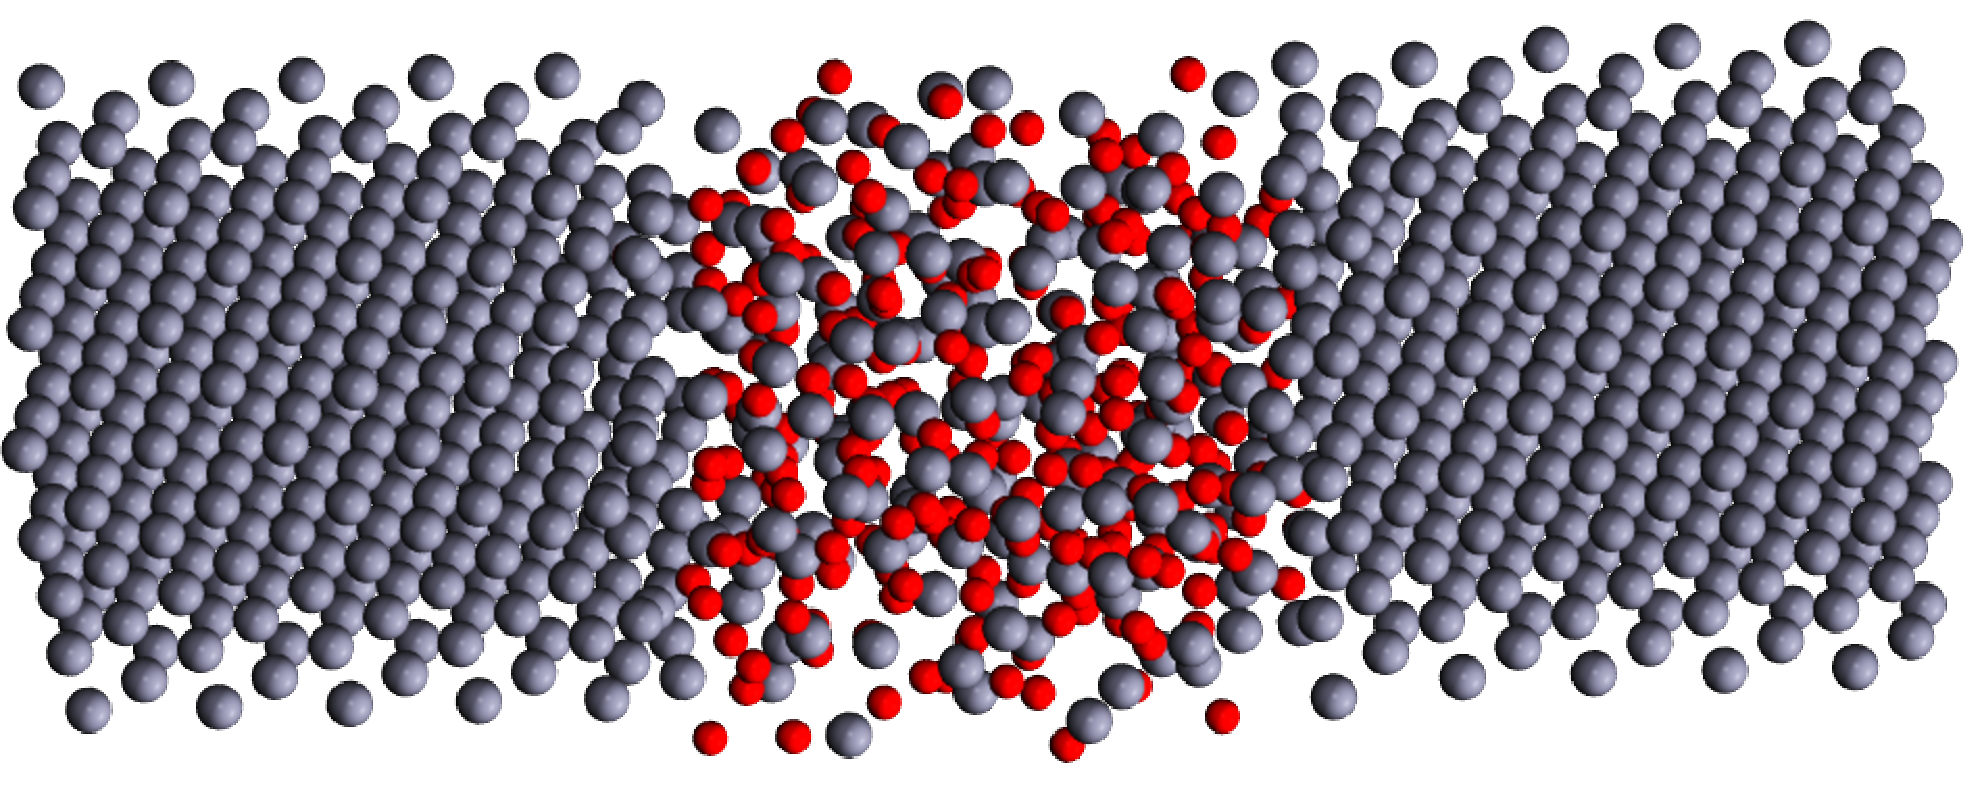
\includegraphics[width=0.9\textwidth]{figures/AlO125_075}
\caption[Atomistic Josephson Junction Model]{\label{fig:povray}Model of a Josephson junction comprised of aluminium \resizebox{!}{0.7em}{
\includegraphics{figures/jjal}} and oxygen \resizebox{!}{0.5em}{
\includegraphics{figures/jjo}}. Two superconducting regions composed only of aluminium, separated by an amorphous AlO$_{1.25}$ barrier with a density 0.75 times that of corundum.}%
\end{figure}

To obtain realistic, high precision atomic positions, computational models of the junction were created using a combination of molecular mechanics and DFT.
A $4\!\times\!4\!\times\!5$ supercell of bulk aluminium (measuring $16.168\times16.168\times20.183$ \AA) representing both the top and bottom slabs was relaxed in the DFT code \sw{VASP}~\cite{Kresse1994, Kresse1996, Kresse1996a} using a projector-augmented wave (PAW) potential~\cite{Kresse1999, Blochl1994}.
Exchange-correlation interactions were evaluated using the PBE functional~\cite{Perdew1996}; a $7\!\times\!7\!\times\!7$ $\Gamma$ centered Monkhorst Pack K point mesh and a plane wave cutoff of $250$ eV.

Formation of the amorphous \ce{AlO_x} layers required a number of preparation steps to accurately represent experimental results.
Corundum was used as a basis for all the constructed junction models as it represents the low temperature and pressure phase of aluminium oxide.
Experimental investigations of stoichiometry suggest, in general, an oxygen deficiency with oxide O/Al ratios varying between 0.6 and 1.4~\cite{Tan2005}, which are highly dependent on the fabrication process.
In response to this, we construct models with four stoichiometries: \ce{AlO_{0.8}}, \ce{AlO_{1.0}}, \ce{AlO_{1.25}} and \ce{AlO_{1.5}}.
The oxide density may also be an important formation variable.
For simplicity we identify oxide density in multiples of the (average) corundum density: $4.05$ g/cm$^\text{3}$, and construct junctions with 0.5, 0.625, 0.75, 0.875 \& 1.0 density multiples for each stoichiometry listed above.
A value of $3.2$ g/cm$^\text{3}$ is typical~\cite{Barbour1998} (which corresponds to a density multiple of 0.8), although theoretical predictions suggest altering the density of this barrier may suppress noise sources of the junction~\cite{DuBois2013}.

Using \ce{AlO_{1.25}} with a density multiple of 0.75 as an example, a $6\!\times\!6\!\times\!1$ supercell of corundum was geometry optimised in the software package \sw{GULP}~\cite{Gale2003}, employing the empirical Streitz-Mintmire potential~\cite{Streitz1994} which can capture the variable oxygen charge states when present in a predominantly metallic environment. This capability is particularly important here, as a Josephson junction has two metal-oxide interfaces.
This large superstructure was required due to the trigonal nature of the lattice, as it was then cut down such that the $xy$ plane of the bulk aluminium slab could be covered.
A non-periodic slab of corundum measuring $16.168\!\times\!16.168\!\times\!11.982$ \AA\ was the result of this process.
Oxygen atoms were randomly removed from the corundum lattice until the appropriate stoichiometry of \ce{AlO_{1.25}} was obtained and the cell was shortened in the $z$-direction to achieve a 0.75 fractional multiple of the corundum density.
These changes add quite a lot of force onto the structure, so a geometry optimisation (in \sw{GULP}) was undertaken at this stage to minimise energy contributions.
To simulate the oxygen deposition phase and generate the amorphous nature of these layers, the structure was then annealed using NVT molecular dynamics at $3000$ K for $3$ µs and quenched to $350$ K over a $1.5$ µs period.

The \ce{AlO_{1.25}} layer was inserted between two bulk Al supercells described above with $0.5$ \AA\ of vacuum space on each side.
The junction was further annealed to simulate a metal--metal--oxide interface reconstruction using \sw{VASP} NVT Molecular Dynamics at $300$ K until equilibrium was reached (approximately $250$ ionic steps), then geometry optimised using a $2\!\times\!2\!\times\!1$ $\Gamma$ centered Monkhorst Pack K point mesh and a $450$ eV plane wave cutoff to obtain the final model, depicted in \cref{fig:povray}.

For comparison, junctions were also modelled without the added computational overhead of DFT by solely employing \sw{GULP} and the Streitz-Mintmire potential.
The construction process of these models matches the procedure above, but interchanges the \textit{ab initio} optimisations of the oxide layer with an empirical framework.

\section{Radial Distribution Function \texorpdfstring{$G(r)$}{G(r)}}\label{sec:gr}
To validate our models against experimental observations, we perform a number of statistical tests to scrutinize the structures.
First we must ensure that the oxide layer of the junctions are in fact amorphous in nature.
We employ a projected radial distribution function
\begin{equation}
G(r) = \lim_{dr \to 0}\frac{p(r)}{4\pi\left(N_{\mathrm{pairs}}/V\right)r^2dr}
\end{equation}
where $r$ is the distance between a pair of particles, $p(r)$ is the average number of atom pairs found at a distance between $r$ and $r + dr$, $V$ is the total volume of the system, and $N_{\mathrm{pairs}}$ is the number of unique pairs of atoms~\cite{Levine2011}.
This function was calculated for each stoichiometry and density configuration using oxygen as the reference species, and aluminium atoms in the amorphous region along with the superconducting bulk as the projection species. \Cref{fig:groptis} depicts the results of this analysis.

\begin{figure}[htp]
\resizebox{0.8\textwidth}{!}{\includestandalone{figures/groptis}}
\caption[Radial Distribution Function]{\label{fig:groptis}Evolution of the oxygen projected radial distribution function $G(r)$. Crystalline corundum \plotline{line width=1pt,color=gray!50}; Metal--oxide interface reconstruction before \plotline{line width=1.5pt,dashdotted, color=Set1-5-3} and after \plotline{line width=1.5pt,dashed, color=Set1-5-2}; final optimised geometry \plotline{line width=2pt,color=Set1-5-1}.}%
\end{figure}

A major peak is visible centered around $1.85$ \AA, which corresponds to convolution of the two Al--O bond distances, $1.852$ \AA\ and $1.971$ \AA\ of the corundum crystal~\cite{Ishizawa1980}.
For a crystalline $G(r)$ this peak is deconvolved to two delta functions (see \cref{fig:groptis} and the discussion below), where here we see a broadening of the statistics and hence differences in neighbour distances: diverging from a crystalline form.
Moving away from this peak to larger distance separations, we see the statistics tending toward a uniform result similar to what a liquid would produce under this analysis.
These two features represent an amorphous system quite well, as close range order suggests a connection to the crystalline form whilst long range order no longer agrees with such periodic conditions.
It's also significant to note that we don't observe neighbours closer than $\sim\!1.5$ \AA\ which is a good indication that the models do not have non-physical neighbour forces acting on atoms.

Most importantly, this trend is almost uniform across all the modeled junctions, which indicate the process outlined in \cref{sec:jjmodel} is capable of producing amorphous oxides whilst varying other physical parameters of the system.
An evolution of the important steps in the procedure is depicted in \cref{fig:groptis}.

The corundum $G(r)$ \plotline{line width=1pt,color=gray!50} is a complicated structure due to the 30 atom unit cell of the crystal, however it is clear from this figure where much of the amorphous structure originates from.
Specifically the $1.852$ \AA\ and $1.971$ \AA\ Al--O bond distance contributions and the void in the $2$--$3$ \AA\ range.
After the melt/quench phase of the procedure \plotline{line width=1.5pt,dashdotted, color=Set1-5-3} the lattice still appears liquid-like.
Whilst the quench cycle minimises the possibility of atoms position very close to one another due to an excess of kinetic energy, it still appears to exhibit liquid behaviour.
This may be a shortcoming of the Streitz-Mintmire potentials ability to capture the relevant physics, however this is rectified after the metal--oxide interface reconstruction is completed \plotline{line width=1.5pt,dashed, color=Set1-5-2} using the \textit{ab initio} methods.
Finally, the geometry optimisation \plotline{line width=2pt,color=Set1-5-1} yields a smoother $1.85$ \AA\ peak and recovers some of the void region around $2$ \AA.

\phantom{push marginfigure}
\begin{marginfigure}
\resizebox{\marginparwidth}{!}{\includestandalone{figures/grcomp}}
\caption[Radial Distribution Function Comparison]{\label{fig:grcomp}Oxygen projected $G(r)$ computed using \textit{ab initio} (\sw{VASP}) \plotline{line width=1.5pt,color=Set1-5-1} and empirical (\sw{GULP}) \plotline{line width=1.5pt,color=Set1-5-2} methods, showing no statistically significant differences.}
\end{marginfigure}
\vspace{-1em}
Whilst optimal $G(r)$ results for both the \sw{VASP} and \sw{GULP} simulations are very similar (\cref{fig:grcomp}), the \sw{GULP} simulation actually produces a drastically different final structure.
We find under \sw{GULP} simulation that stoichiometric ratios higher than 1:1 are not stable and oxygen atoms diffuse into the metallic regions until a stoichiometric ratio of at most 1:1 is achieved.
As a result of this excess oxygen diffusion, the junction width can increase by up to 30\% or more over the course of the simulation.
At high densities and stoichiometries (than typical amorphous alumina) some expansion of the oxide region is also seen in the \textit{ab initio} simulations, although this effect is much less pronounced.
Higher oxygen mobility in \sw{GULP} could be attributed to shortcomings of the empirical potential, but we see very little increase in oxide distribution during the optimisation phase -- suggesting that the details of the Nos\'{e}-Hoover thermostat routine employed during the MD simulation may play a role.

\section{Total Energy and Optimal Conditions}
The total energy of a computational model is a good indication of the structures' electronic stability.
Due to the stoichiometry changes invoked in the oxygen depleted models, not all structures have the same number of atoms.
This gives structures with more atoms (such as \ce{AlO_{1.25}}) additional electronegativity which in turn results in a deeper potential well and a large total energy.
In an attempt to normalise this response, we present a total energy per atom value in \cref{fig:energyperatom}, scaling against stoichiometry (left) and density (right).

\begin{figure}[tbp]
\peratommargins
\begin{adjustwidth}{\peratomleft}{\peratomright}
\resizebox{\widefigure}{!}{\includestandalone{figures/energyperatom}}
\caption[Energy Comparisons]{\label{fig:energyperatom}Total energy per atom for various junction models with stoichiometry (left) and density (right).  Although the total energy per atom is strongly dependent on stoichiometry, we see a clear tread to optimal densities of approximately 75\% of the density of corundum.}
\end{adjustwidth}
\end{figure}

It is clear from this figure that stoichiometry plays a larger role in energy minimisation than density, and that the structures would prefer additional oxygen to minimise internal forces.
This suggests that fabrication processes that generate oxygen deficiencies may be inviting the inclusion of alien species or oxygenic site hopping in an attempt to rectify this offset.

Density changes seem to alter the energy contribution marginally.
Minimum energies correspond to density multiples between 0.6 and 0.75 -- slightly lower than typical constructions of $3.2$ g/cm$^\text{3}$~\cite{Barbour1998} (an 0.8 density multiple); which may indicate another method of experimentally optimising the junction formation process.

\section{Coordination Number}\label{sec:coord}
Coordination number is a useful metric which allows for some insight into both the crystallinity of the structures being analysed, and their similarity to fabricated junctions. For instance, in the corundum structure every aluminium ion is coordinated with six oxygen ions. In amorphous alumina, the proportion of 6-coordinated aluminium as compared to 4-coordinated aluminium is an experimentally accessible quantity and has been reported on previously~\cite{ElMashri1983}. However, in order to establish this ratio it is assumed that there is a bimodal distribution of hexahedral (\ce{AlO_6}) and tetrahedral (\ce{AlO_4}) coordination. Ratios of \ce{AlO_6}:\ce{AlO_4} are quoted in a range from 80:20 to 30:70, depending on the method by which the oxide layer was formed~\cite{Bourdillon1984}. More modern techniques using Nuclear Magnetic Resonance (NMR) are also able to resolve any \ce{AlO_5} coordinations~\cite{Lee2009}.\nomdef{ANMR}{NMR}{Nuclear Magnetic Resonance}


\begin{figure}[htp]
\centering
\resizebox{\textwidth}{!}{\includestandalone{figures/coord_hists}}
\caption[Oxygen Coordination]{\label{fig:coordinationnumber}Distribution of oxygen coordination about aluminium as a function of density and stoichiometry, showing a tendency to higher coordination number with increasing density or stoichiometry.}%
\end{figure}

\Cref{fig:coordinationnumber} shows the distribution of oxygen coordination about aluminium as a function of density and stoichiometry. These results are calculated using an Al--O bond length cutoff of $2.5$ \AA, which corresponds to the first minimum after the nearest neighbour peak in the $G(r)$ (see \cref{fig:groptis}). As one would expect, the coordination number (for Al--O bonding) increases with increasing density or stoichiometry. We also note that there exists a reasonable proportion of $2$- and $3$-coordinated aluminium atoms, which persists at high density and stoichiometry. In order to compare directly to previous experimental and theoretical work, we compute the ratio of $4$-, $5$- and $6$-coordination for Al--O bonding, matching the stoichiometry of 1.5 and assuming the density multiple closest to experimental values (0.750). The results are presented in \cref{tab:coord_comp}. We observe excellent agreement, both before and after the \textit{ab initio} optimisation.

\begin{table}[h]
\caption[Aluminium coordinations]{\label{tab:coord_comp} Relative proportions of $4$-, $5$- and $6$-coordinated aluminium atoms within the oxide layer for a density of 0.75 and stoichiometry of 1.5.}
\centering
\begin{tabular}{ @{}lccc } \toprule
 & $4$ (\%) & $5$ (\%) & $6$ (\%) \\ \midrule
\sw{VASP} (before optimisation)	& $57$ & $39$ & $4$ \\
\sw{VASP} (after optimisation)	& $53$ & $43$ & $4$ \\
\citeauthor{Lee2009} \cite{Lee2009}; experiment	& $55 \pm 3$ & $42 \pm 3$ & $3 \pm 2$ \\
\citeauthor{Momida2011} \cite{Momida2011}; theory   & $60.4$ & $29.2$ & $10.4$ \\ \bottomrule
\end{tabular}
\end{table}

\section{Chapter Summary}\label{sec:jjsum}

Precise computational models of Josephson junctions are becoming crucial to efforts to reduce dissipation and loss in superconducting circuits.
The limits of computational resources mean that full \textit{ab initio} models are computationally intractable.
However, a combination of \textit{ab initio} and empirical models holds promise for developing flexible and efficient simulation approaches.
Through comparisons with both previous theoretical analysis and experimental measurements, we have shown that the resulting structures are representative of those fabricated experimentally.
The structure of such junctions may now be used as input conditions for the delocalised oxygen models discussed in the subsequent chapters.
Additionally, free parameters in existing phenomenological defect models can be determined via information directly obtained from the atomic positions, and other microscopic TLS models may use these structures to investigate their own particular phenomenon.


    %\versoquote{When a person is determined to believe something, the very absurdity of the doctrine confirms them in their faith.}{Junius}
\chapter{Microscopic TLS Model}\label{ch:tls}
\chapterprecis{The Microscopic TLS Model chapter}%TODO: Fill this in.
\loftchap{Microscopic TLS Model}

\section{Concept and background}
\section{Potential configuration}

\begin{equation}
    H = -\frac{\hbar^2}{2m_{oxy}}\nabla^2+V(\mathbf{r})
    \label{eq:OHam}
\end{equation}

\begin{table}[h]
\caption[Streitz-Mintmire Pair Constants]{\label{tab:smconsts} Empirical constants used in the calculation of the Buckingham and Rydberg pair potentials in the Streitz-Mintmire formalism~\cite{Streitz1994,Gale2003}.}
\centering
\begin{tabular}{ c*{5}{r@{.}l} } \toprule
Pair & \multicolumn{2}{c}{A} & \multicolumn{2}{c}{$\rho$} & \multicolumn{2}{c}{B} & \multicolumn{2}{c}{C} & \multicolumn{2}{c}{$r_0$}  \\ \midrule
Al--Al & 4&474755 & 0&991317 & 0&159472 & 5&949144 & 3&365875 \\
Al--O & 62&933909 & 0&443658 & 0&094594 & 9&985407 & 2&358570 \\
O--O & 3322&784218 & 0&291065 & 1&865072 & 16&822405 & 2&005092 \\ \bottomrule
\end{tabular}
\end{table}

\begin{figure}[htp]
\centering
\resizebox{0.8\columnwidth}{!}{\includestandalone{figures/mexhatproj}}
\caption[Potential Projections]{\label{fig:mexhatproj}\lin{1D} double wells (blue, solid) and harmonic wells (red, dashed) can be used to represent simple projections of a \lin{2D} potential onto the $x$ and $y$ axes. Left: two projected double wells is an example of a tetra-well. Right: a combination of one double well and a harmonic well reflects the hemi-tetra- case.}
\end{figure}

\section{Solving Derivatives Numerically}\label{sec:numder}
The Streitz Mintmire potential \cite{Streitz1994} is an assemblage of many functional forms and integrals, which in total are not completely analytic over all regions of importance.
Therefore $\nabla^2$ in \cref{eq:OHam} will also require numerical treatment over a discrete grid of spatial coordinates.
A number of methods exist for this problem; most of which introduce errors from various approximations and platform limitations.
Models exist that effectively remove these errors, but are usually incredibly mathematically complex and problem specific: for example, a variational model which calculates an optimised three-finite-burn lunar escape trajectory~\cite{Ocampo2012}.

On the simpler end of the spectrum, finite difference algorithms are useful for boundary value problems (where forward and backward methods are usually applied), and for ordinary and partial differential equations.
If a first order ODE (or PDE) of the form $f(x)$ can be evaluated both left and right of $x$, the central difference method can be used where absciss\ae\ are chosen symmetrically about $x$, which takes the form
\nomdef{AODE}{ODE}{Ordinary Differential Equation}
\nomdef{APDE}{PDE}{Partial Differential Equation}
\begin{equation}
f\,'(x) \approx \frac{f(x+h)-f(x+h)}{2h},\label{eq:simplecdiff}
\end{equation}

where $h$ is some step size.
\nomdref{CSTEP}{h}{A step size used in the central difference formalism}{ch:tls}
The step size controls the accuracy of the computed derivative, which is unfortunately bound by two factors.
If the step size is too small, numerical roundoff errors cause accuracy issues; on the other hand, step sizes which are too large see mathematical truncation errors dominate.
Identifying an optimal balance for the step size is also dependent on the specific value of $f\,'(x)$ being calculated, which may not be appropriate for a similar set of values.
This problem, known as `the step size dilemma' has generated a number of investigations in an attempt to find a middle ground between simple finite difference methods with strong bounding conditions and the highly domain specific models like the variation model described above.

The complex step method (exploiting complex perturbations of the general Taylor series) yields no subtractive cancellation errors (\emph{vide infra} \cref{subsec:roundoff})~\cite{Squire1998}, which exist in the real spaced Taylor series finite difference methods; \cref{eq:simplecdiff} is a simple example of this.
However, for many years this statement was only true for the first order derivative -- higher orders were shown to have as many cancellation errors as their finite difference counterparts.
This method was therefore excluded as a candidate for the model constructed for this thesis, as it would perform on par with standard finite difference methods for the second order derivative we wish to compute.
After much of the base code for this model had been constructed, a generalised, arbitrary order derivative complex step algorithm was published~\cite{Lantoine2012}.
This algorithm may improve the error contribution of the models' final implementation, although this has not been investigated.

A second possible successor to finite difference is automatic differentiation (AD).
\nomdef{AAD}{AD}{Automatic Differentiation}
The premise of this algorithm isn't necessarily mathematical in nature, but capitalises on the fact that computers are methodological reductionists and ultimately only execute simple arithmetic operations no matter how complicated the actual computation is.
Repeatedly applying the chain rule to these operations, AD can compute the derivative to working precision~\cite{Kedem1980}.
There a two methods to implement this algorithm; neither is straightforward.
One uses special AD preprocessors that analyse each function call, break it up instruction by instruction and generates a new function that computes derivatives.
Method two involves operator overloading that can generate code at compile time, which in a JIT accelerated environment like \texttt{Matlab} is unfeasible -- requiring some hacking of the engine itself.
\nomdef{AJIT}{JIT}{Just-in-time compilation}

Both AD and complex step require access to functions at the source code level, meaning calls to third party libraries like \texttt{BLAS} and \texttt{LAPACK} (which are used in this model's implementation \xxx{section on lapack}) become increasingly over-complicated.

For these reasons, it was decided to implement our model using a finite central difference method, paying close attention to the inherent error in exchange for relative computational simplicity.

\section[Understanding Central Differences]{Understanding the Central Difference Method\footnote{While most of this and the following section is standard cannon information for finite differences; it closely follows sections of \citeauthor{Mathur2012}~\cite{Mathur2012}, which will be formally introduced in \cref{sec:hopt}.}}\label{sec:ucdiff}

All finite difference methods involve truncating a Taylor series expansion of a function $f(x)$ about $x^*$ after a certain number of terms\nomdref{CxStar}{$x^*$}{Any value of $x$ about which a central difference is applied}{ch:tls}
\begin{equation}
    f(x) = f(x^*) + f^{\;\prime}(x)(x-x^*) + \cdots + R_n.
\end{equation}

The discarded, higher order remainder terms $R_n$, are considered to contribute a negligible error to the approximation assuming a sufficiently small step size $h$.\nomdref{CRn}{$R_n$}{High order remainder terms of a Taylor series expansion of $f(x)$ to be truncated when using central difference}{sec:ucdiff}
\begin{equation}
    R_n = \sum_{m=n}^\infty \frac{f^{\;(m)}(x^*)}{m!}(x-x^*)^m
\end{equation}

It can be shown using the integral calculus derivation of the Taylor series that the $d^{th}$ derivative can be bound over the interval $[x^*, x]$, \ie $a\leq f^{\;(d)}(x) \leq~c$ \cite{Greenberg1978}.
Furthermore, $\exists b \in [a,c]$ such that the remainder can be written as
\begin{equation}
   R_d = b \frac{(x-x^*)^d}{d!}.
\end{equation}

The Intermediate Value Theorem can be invoked at this stage to posit some point $\xi \in [x^*,x]$ exists for which $f^{\;(d)}(\xi)$ will equal the unknown parameter $b$.
$R_d$ in this form is called the Lagrange remainder.\nomdref{Xd}{$(d)$}{The $d^{th}$ derivative used in central difference methods}{ch:tls}\nomdref{Zn}{$n$}{The $n^{th}$ order expansion of the Taylor series used in central difference methods}{ch:tls}
While there is no known method to determine a value of $\xi$ exactly for a general function, it is useful to express the $d^{th}$ order Taylor series in terms of the Lagrange remainder:
\begin{equation}
    f(x) = \sum_{k=0}^d \frac{f^{\;(k)}(x^*)}{k!}(x-x^*)^k + \frac{f^{\;(d+1)}(\xi)}{(d+1)!}(x-x^*)^{d+1}, \quad \xi \in [x^*,x].\label{eq:taylorrem}
\end{equation}

The most commonly used central difference formula is the first derivative of second order, which can be obtained by applying \cref{eq:taylorrem} at two absciss\ae\ of length $h$ from a sampling point in $f(x)$ and solving the simultaneous equation for $f^{\;\prime}(x)$.
\begin{align}
f(x+h) &= f(x) + f^{\;\prime}(x)h + \frac{f^{\;\prime\prime}(x)}{2}h^2 + \frac{f^{\;(3)}(\xi^+)}{2}h^3, \quad \xi^+ \in [x,x+h] \\
f(x-h) &= f(x) - f^{\;\prime}(x)h + \frac{f^{\;\prime\prime}(x)}{2}h^2 - \frac{f^{\;(3)}(\xi^-)}{2}h^3, \quad \xi^- \in [x-h,x] \\
f^{\;\prime}(x) &= \frac{f(x+h)-f(x-h)}{2h} - \frac{f^{\;(3)}(\xi^+)+f^{\;(3)}(\xi^-)}{2}\frac{h^2}{3!}\label{eq:cd12pm}
\end{align}

The error term in \cref{eq:cd12pm} contains the average of the third derivative evaluated the two unknown points $\xi^+$ and $\xi^-$, which are bounded inside the range $[x-h,x+h]$.\nomdref{Goxi}{$\xi$}{An unknown but bounded point used in central difference methods}{ch:tls}
Applying the Mean Value Theorem and assuming that $f^{\;(3)}(x)$ is smooth over the bounded range, a value $\xi$ must exist between $\xi^+$ and $\xi^-$ which satisfies the average.
\begin{align}
f^{\;\prime}(x) &= \frac{f(x+h)-f(x-h)}{2h} - \frac{f^{\;(3)}(\xi)}{3!}h^2, \quad \xi \in [x-h,x+h]\label{eq:cd12t} \\
\mathcal{F}_2^{\,(1)}(x,h) &= \frac{f(x+h)-f(x-h)}{2h} + \mathcal{O}(h^2)\label{eq:cd12f}
\end{align}

Both equations above represent the first derivative of $f(x)$; although they differ in the sense that \cref{eq:cd12t} is still the true derivative and \cref{eq:cd12f} truncates the error term and represents it as an order of magnitude -- which is the essence of the finite difference approximation to the derivative.
The notation $\mathcal{F}_n^{\,(d)}(x,h)$ represents the general form of the approximation of the $d^{th}$ derivative of $f(x)$ of order $n$ using step size $h$, which can formerly be expressed as:\nomdref{CFD}{$\mathcal{F}_n^{\,(d)}(x,h)$}{Finite difference approximation of the $d^{th}$ derivative of $f(x)$ of order $n$ using step size $h$}{ch:tls}\nomdef{BO}{$\mathcal{O}$}{Big-O notation, signifying the order of a value}
\begin{equation}
\mathcal{F}_n^{\,(d)}(x,h) = \frac{\Delta f_n^{\;(d)}(x,h)}{h^d} + \mathcal{O}(h^n).\label{eq:cdgeneral}
\end{equation}

The $\Delta f_n^{\;(d)}$ term describes the appropriate finite difference expression obtained from the set of \cref{eq:taylorrem} for particular values of $n$ and $d$.
Frequently used constructions of this form can be found in tables in books such as \citeauthor{Mathews2004} and web resources like \citeauthor{Holoborodko2009} without the need to derive them from first principles, although comprehensive error discussion is uncommon or oversimplified at best~\cite{Mathews2004,Holoborodko2009}.

Solving the Schr\"{o}dinger equation using the hamiltonian \cref{eq:OHam} requires a second derivative finite difference expression.
Truncating the Taylor series at $\mathcal{O}(h^2)$ is the simplest arrangement, which takes the form
\begin{equation}
f^{\;\prime\prime}(x) = \frac{f(x-h)-2f(x)+f(x+h)}{h^2} - \frac{f^{\;(4)}(\xi)}{12}h^2, \quad \xi \in [x-h,x+h]\label{eq:cd22t} \\
\mathcal{F}_2^{\,(2)}(x,h) = \frac{f(x-h)-2f(x)+f(x+h)}{h^2} + \mathcal{O}(h^2).\label{eq:cd22f}
\end{equation}

Before applying this method, a step size must be chosen; which relies on an accurate description of the competing error contributors.

\section{Contributors to the Step Size Dilemma}

\subsection{Truncation Error}\label{sec:truncerr}

The truncation error in \cref{eq:cd22f} as $h\!\to\!0$ is not surprisingly $\mathcal{O}(h^2)\!\to\!0$, implying that $h$ should be as small as possible to maximise the accuracy of the calculation.
Limits can also be put on the true truncation error as well.
Even though $\xi$ is an unknown quantity, as the step size decreases, so does range in which $\xi$ exists.
Hence the limit of \cref{eq:cd22f} becomes
\begin{equation}
\lim_{h \to 0}\mathcal{O}(h^2) =  - \frac{f^{\;(4)}(x)}{12}h^2.
\end{equation}

This error differs for each formula, depending on the particular values of $n$ and $d$ (for example, the error in \labelcref{eq:cd12t} tends to $\cramped{-\frac{f^{\;(3)}(x)}{3!}h^2}$).
Using \cref{eq:cdgeneral} and \cref{eq:cd22f}, a general relationship between the true $d^{th}$ derivative and its finite difference approximation\nomdref{CFDT}{$f_n^{\;(d)}(x)$}{True $d^{th}$ derivative of $f(x)$ of order $n$ expressed in terms of a finite difference approximation}{ch:tls}
\begin{equation}
 f_n^{\;(d)}(x) = \mathcal{F}_n^{\,(d)}(x,h) + C(x,h)h^n,\label{eq:cdadj}
\end{equation}

can be expressed with an undetermined truncation coefficient term $C(x,h)$, which is independent of the derivative parameter $d$.
This coefficient represented in Lagrange form is
\begin{equation}
C(x,h) = a_1\,f_n^{\;(n+d)}(\xi), \quad \xi \in [x-a_2h,x+a_3h],\label{eq:cdcxh}
\end{equation}

with the set of unknown constants $a$ also being dependent on the finite difference formula in question.
As the truncation coefficient's is dependent on $\xi$, its dependence on $h$ is removed as $h\!\to\!0$ (because $\xi\!\to\!x$).
Hence, for small values of $h$, a simplified coefficient can be defined as
\begin{equation}
 C_n(x) \equiv a_1\,f_n^{\;(n+d)}(x).
\end{equation}

Simplifying \cref{eq:cdadj} with this new coefficient, it is clear that this relationship takes the form of a Richardson extrapolation, therefore we can evaluate at two different step sizes $h_1$ and $h_2$ (where $h_1 > h_2$)
\begin{align}
f_n^{\;(d)}(x) &= \mathcal{F}_n^{\,(d)}(x,h_1) + C_n(x)h_1^n \\
f_n^{\;(d)}(x) &= \mathcal{F}_n^{\,(d)}(x,h_2) + C_n(x)h_2^n
\end{align}

and solving for $C_n(x)$ we find\nomdref{CCn}{$C_n$}{Approximate truncation coefficient for small step sizes. Expands to $C_n(x,h)$ for all steps}{ch:tls}
\begin{equation}
 C_n = \frac{\mathcal{F}_n^{\,(d)}(x,h_2) - \mathcal{F}_n^{\,(d)}(x,h_1)}{h_1^n - h_2^n}.\label{eq:cdtrcoeff}
\end{equation}

This expression still assumes a small step size such that the approximated truncation coefficient stays independent of $h$ (and therefore constant for a valid range of steps).
The complete estimate for the truncation error of order $n$ can now be found via \cref{eq:cdadj}\nomdref{BTEn}{$\mathcal{TE}_n(x,h)$}{Truncation error of order $n$ for central difference methods}{sec:truncerr}
\begin{equation}
\mathcal{TE}_n(x,h_1) = C_n h_1^n = \frac{\mathcal{F}_n^{\,(d)}(x,h_2) - \mathcal{F}_n^{\,(d)}(x,h_1)}{h_1^n - h_2^n}h_1^n.\label{eq:cdte}
\end{equation}

As much of this derivation requires a `sufficiently small' step size, it's imperative to consider the behaviour of the truncation error at larger values of $h$ as well.
If $h$ increases, the approximate truncation coefficient can no longer be used and
the magnitude of the true coefficient $C(x,h)$ may become very large and unwieldily as there is no restriction of the values over $f^{\;(n+d)}(x\pm h_{large})$.
Additionally, $h^n$ in \cref{eq:cdte} increases, ultimately suggesting that a step size `too large' will also result in unpredictable truncation error values.

\subsection{Roundoff Errors}\label{subsec:roundoff}

As mentioned in \cref{sec:numder}, numbers in a computer are represented with a fixed number of binary digits, and operations applied to them have an inherent loss of accuracy.
This phenomenon is designated the term roundoff error, as the extra digits that cannot be held in memory must be discarded -- rounded to the nearest tolerance.

Roundoff error has been a hot topic of research since the invention of computers.
Notable checks on the accuracy of finite element methods were completed before the moon landings~\cite{Cyrus1968} and investigations after a Patriot missile defense system allowed a Scud missile to hit a barracks, killing 28 people; found roundoff via the differencing of floating point numbers introduced errors into the timing register when converting representations~\cite{Skeel1992}.
These relative errors caused by subtraction (called cancellation error) tend to decrease as $h$ is increased, thus to minimise this uncertainty $h$ should be as large as possible -- contrary to the truncation requirement of a small step size.
An upper bound on this error is given by
\begin{equation}
 \abs{(\alpha-\beta)_{true} - (\alpha-\beta)} \leq \delta \max(\abs{\alpha},\abs{\beta}),
\end{equation}

where $\alpha$ and $\beta$ are two fixed precision numbers, and $\delta$ indicates the precision of the calculation.
Usually, modern computer languages operate using standard double precision floating point numbers, thus $\delta = 2^{-53}$.\nomdref{Gd}{$\delta$}{Precision of a calculation using floating point numbers. On modern computers using double precision $\delta = 2^{-53}$}{ch:tls}

A second roundoff error type known as condition error creeps in when functions don't use machine precision floating point numbers in their internal routines.
For example, a third party function may approximate π to 3.14159, which would artificially round the result of whatever operation was being applied to a precision of $10^{-5}$.
As with cancellation error, an upper bound can also be formulated for condition error:
\begin{equation}
\abs{f(x)_{true} - f(x)}\leq \epsilon \abs{f(x)}.
\end{equation}

Here, $\epsilon$ is the magnitude of the most significant digit affected by the condition error.\nomdref{Ge}{$\epsilon$}{Magnitude of the most significant digit affected by condition error}{ch:tls}
For elementary operations $\epsilon$ should be equal to machine precision, although this cannot be assumed for all functions hence it is a value that should be calculated in general.

Finally, an error which is also important in this instance is named representational error.
Not all numbers can be accurately be represented in binary using a fixed number of digits.
Many people choose their step sizes in base 10 (\eg $1\ten{-2}$, $5\ten{-6}$ \etc), and what's most troubling about this is the fact that no negative power of 10 has an exact binary representation.
This error is small -- usually smaller that machine precision in fact, but it has non-trival and cumulative side effects.
If one avoids step sizes other than $2^\mathds{N}$ this error can be avoided completely.

With this information in hand, an upper bound to the total roundoff error can now be calculated:
\begin{equation}
 \abs{\mathcal{F}_n^{\,(d)}(x,h)_{true}-\mathcal{F}_n^{\,(d)}(x,h)} \leq \frac{\epsilon\abs{\mathcal{F}_\epsilon}+\delta\abs{\mathcal{F}_\delta}}{h^d}.
\end{equation}

The functions $\mathcal{F}_\epsilon$ and $\mathcal{F}_\delta$ are derived from $\Delta f_n^{\;(d)}$ (see \labelcref{eq:cdgeneral}).
Forms of \cref{eq:cd22f} for instance are\nomdref{BFE}{$\mathcal{F}_\epsilon$}{Condition error coefficient for central difference methods}{ch:tls}\nomdref{BFD}{$\mathcal{F}_\delta$}{Cancellation error coefficient for central difference methods}{ch:tls}
\begin{align}
\mathcal{F}_\epsilon &= \abs{f(x+h)} + \abs{2f(x)} + \abs{f(x-h)} \\
\mathcal{F}_\delta &= \max(\abs{f(x+h) + f(x-h)},\abs{2f(x)}).
\end{align}

\subsection{Estimation of Total Error}\label{subsec:cdtoterr}

Using the equations for truncation and roundoff errors mentioned above, and assuming a small $h$ such that \cref{eq:cdtrcoeff} holds, the total error can be bounded by the expression
\begin{equation}
\abs{f^{\;(d)}(x)_{true}-\mathcal{F}_n^{\,(d)}(x,h)} \leq \frac{\epsilon\abs{\mathcal{F}_\epsilon}+\delta\abs{\mathcal{F}_\delta}}{h^d} + \abs{C_n}h^n
\end{equation}

Assuming a worse case scenario, the total error can therefore be described as\nomdref{BEnd}{$\mathcal{E}_n^{\,(d)}(x,h)$}{Total error for a $d^{th}$ derivative central difference method of order $n$}{subsec:cdtoterr}
\begin{equation}
\mathcal{E}_n^{\,(d)}(x,h) = \frac{\epsilon\abs{\mathcal{F}_\epsilon}+\delta\abs{\mathcal{F}_\delta}}{h^d} + \abs{C_n}h^n\label{eq:cnetot}
\end{equation}

noting the dependence on $x$ comes from the functions $\mathcal{F}_\epsilon$ and $\mathcal{F}_\delta$, and that $\epsilon$ is still an unknown value.

\section{Calculating an Optimal Step Size}\label{sec:hopt}

With all of these caveats in mind, finding an optimal step size $h_{opt}$ is a troublesome undertaking; which is why the complex step and AD methods discussed in \cref{sec:numder} were developed.

A simple method proposed in \citeauthor{Gill1982} suggests minimising an expression similar to \cref{eq:cnetot} which trades off the truncation and roundoff errors ~\cite{Gill1982,Mathews2004}.
However, this method assumes the condition error $\epsilon$ is known and cancellation error is treated in a trivial manner.

Violation of monotonicity is an algorithm which attempts to ignore actually calculating any estimates for truncation and roundoff errors~\cite{Stepleman1979}. This method breaks down if \cref{eq:cdtrcoeff} doesn't hold and therefore is not a general solution.

Algorithms specifically designed for forward differences have also been discussed in the literature~\cite{Barton1992}, but are of no benefit for purposes herein.

The method which has been chosen to be implemented in this work is the algorithm from the PhD thesis of \textbf{Ravishankar Mathur}, which allows one to calculate an optimal step without \emph{a priori} knowledge of the condition error $\epsilon$.
Additionally, corrections to the the step size are introduced to account for the approximate nature of the truncation coefficient $C_n$, as well as estimations of step size validity and the maximal appropriate step size for a problem are examined~\cite{Mathur2012}.

As with \citeauthor{Gill1982}, \citeauthor{Mathur2012} starts by minimising the total error expression
\begin{equation}
\frac{\partial\mathcal{E}}{\partial h} = -d\frac{\epsilon\abs{\mathcal{F}_\epsilon}+\delta\abs{\mathcal{F}_\delta}}{h^{d+1}} + n\abs{C_n}h^{n-1} = 0
\end{equation}

and solving for $h$ to find
\begin{equation}
h_{opt,\mathcal{TE}} = \left[\frac{d}{n}\frac{1}{\abs{C_n}}\left(\epsilon\abs{\mathcal{F}_\epsilon}+
\delta\abs{\mathcal{F}_\delta}\right)\right]^{1/(n+d)}.\label{eq:cdhopt}
\end{equation}

Note that obtaining correct values of $\mathcal{F}_\epsilon$ and $\mathcal{F}_\delta$ require the optimal step size $h_{opt,\mathcal{TE}}$, thus an iterative method is required.
Once this value is known, \cref{eq:cdhopt} can be rearranged to find the condition error $\epsilon$.

The steps of the algorithm which computes these values (as well as discussions of further optimisations) can be found in Chapter 3 of~\,\onlinecite{Mathur2012}.

\subsection{A Harmonic Approximation to Streitz Mintmire}\label{subsec:harmsm}

A complication arises when attempting to apply this algorithm to $\nabla^2$ in \cref{eq:OHam}, which more specifically should be written as $\cramped{\frac{\mathrm{d}^2\Psi}{\mathrm{d}x^2}}$; where $\Psi(x)$ is an eigenstate of $H$ in the time-independent Schr\"odinger equation $H\ket{\Psi(x)} = E\ket{\Psi(x)}$.\nomdef{CH}{$H$}{The Hamiltonian operator, corresponding to the total energy of a system}\nomdef{CE}{$E$}{Energy of a system}\nomdef{BPsi}{$\Psi_n(x)$}{$n^{th}$ state wavefunction}
This eigenvalue equation is solved via direct diagonalisation of the hamiltonian matrix - requiring a descretised treatment of $\nabla^2$ before $\Psi(x)$ can be obtained.
The step size algorithm requires an analytical form of the function to which it is applied.
Unfortunately there are very few quantum mechanical systems with analytical solutions, and from that small pool, most are overly simplified constructions that do not exist physically.
The functional form of the wavefunction for a particle under the influence of the Streitz Mintmire potential is not one of these systems.
However, certain configurations of the potential approximate to a parabola-like shape (see section \xxx{Add in the mex hat section}x, \cref{fig:mexhatproj} and \cref{fig:smvh}) -- which has a simple analytic solution in the frame of\xxx{just for you Jared} the quantum harmonic oscillator that can serve as an analogue in this limit.

The hamiltonian of a particle in a one dimensional quantum harmonic oscillator can be described as
\begin{equation}
\widehat{H} = \frac{\widehat{p}^2}{2m}+\frac{1}{2}m\omega^2\widehat{x}^2\label{eq:hamho}
\end{equation}

where $m$ is the particle's mass and $ω$ is the angular frequency of the oscillator.\nomdef{Cmass}{$m$}{Mass of a particle}\nomdef{Gz}{$\omega$}{Angular frequency}
Two operators, $\widehat{x} = x$ for position and $\cramped{\widehat{p} = -i\hbar \frac{\partial}{\partial x}}$ for momentum describe the complete Schr\"{o}dinger equation.
After separation of variables, the time independent form becomes
\begin{equation}
-\frac{\hbar^2}{2m}\frac{\partial^2 \Psi}{\partial x^2}+\frac{1}{2}m\omega^2x^2 \Psi = E\Psi,
\label{eq:hamti}
\end{equation}

with the family of solutions for the wavefunctions\nomdef{Bhbar}{$\hbar$}{Reduced Planck constant, $\hbar \simeq 1.055\ten{-34}$ Js}
\begin{align}\psi_n(x) &= \frac{1}{\sqrt{2^n\,n!}}\left(\frac{m\omega}{\hbar\pi}\right)^{1/4}e^{
- \frac{m\omega x^2}{2 \hbar}} H_n\left(\sqrt{\frac{m\omega}{\hbar}} x \right), &n = 0,1,2,\ldots \\
H_n(x) &= (-1)^n e^{x^2}\frac{\mathrm{d}^n}{\mathrm{d}x^n}\left(e^{-x^2}\right) \\
\therefore \psi_0(x) &= \left(\frac{m\omega}{\hbar\pi}\right)^{1/4}e^{
- \frac{m\omega x^2}{2 \hbar}} \label{eq:gshwfn}
\end{align}

where $\psi_0(x)$ \cref{eq:gshwfn} is the ground state wavefunction. Particle mass $m$ in our case is the mass of an oxygen atom, and the angular frequency $\omega$ is currently unknown.

Using a small step size, the eigenvalue equation is solved for the Streitz Mintmire case, and a ground state wavefunction is found.
The functional form of which is shown in the left plot of \cref{fig:smvh} as \plotline{line width=1.5pt,color=Set1-5-1}.
As the potential form (shown in the right plot) is similar to a parabola, the resultant wavefunction is gaussian-like.
Using \cref{eq:gshwfn}, a harmonic form of the ground state wavefunction can now be fitted to the calculated Streitz Mintmire result through the unknown angular frequency, which is found to be $\omega = 2.241\ten{13}$ rad/s.
Both $\psi_0(x)$ and the associated potential of this harmonic approximation are plotted as \plotline{line width=1.5pt,color=Set1-5-2} to compare with the Streitz Mintmire result.
\begin{figure}[htp]
\centering
\resizebox{\widefigure}{!}{\includestandalone{figures/smvh}}
\parbox{\widefigure}{\caption[Harmonic Approximation to Strietz Mintmire]{\label{fig:smvh}Calculated Streitz Mintmire \plotline{line width=1.5pt,color=Set1-5-1} and Harmonic approximations \plotline{line width=1.5pt,color=Set1-5-2} to the ground state wave function $\psi_0(x)$ (left) and potential $V(x)$ (right). The harmonic response is scaled via $\omega = 2.241\ten{13}$ rad/s using \cref{eq:gshwfn}. Units of $V(x)$ in [μeV] with $x$ in [Å] correspond to length scales of experimental results.}}
\end{figure}

The fitted value of $\omega$ yields a complete approximation to the Strietz Mintmire ground state wavefunction, which we can now use in conjunction with \cref{eq:cd22f} to compute $\nabla^2$ in \cref{eq:OHam}; evaluating at $x = 0$ to find the eigenvalue $E$.

\Cref{fig:hopt3pt} displays the absolute value of the truncation error \cref{eq:cdte} over a range of possible step sizes \plotmarker{0.4}{circle,fill=Set1-5-2}.
Roundoff errors dominate for small step sizes ($h \lesssim 5\ten{-5}$) with some step sizes resulting in completely invalid results (\ie $\mathcal{TE}_2 = 0$).
These steps are labelled \plotmarker{0.25}{regular polygon, regular polygon sides=3,fill=Set1-5-2} and are scaled to $2\ten{-8}$ to be displayed on the graph.
As the step size increases, truncation error dominates until the region $h \gtrsim 5$, where this error becomes invalid.
\begin{figure}[htp]
\centering
\resizebox{\columnwidth}{!}{\includestandalone{figures/hopt3pt}}
\caption[Step size optimisation of $f_2^{\;(2)}(x)$]{\label{fig:hopt3pt}Step size optimisation of $f_2^{\;(2)}(x)$ for step sizes $10^{-9}\!\leq\! h\! \leq\! 10^1$ \plotmarker{0.4}{circle,fill=Set1-5-2}. Steps which generate an invalid roundoff error (\ie $\mathcal{TE}_2 = 0$) are translated to $2\ten{-8}$ for display purposes and labelled \plotmarker{0.25}{regular polygon, regular polygon sides=3,fill=Set1-5-2}. Two optimal step sizes are identified: $h_{opt,\mathcal{TE}}$ \plotmarker{0.5}{circle,fill=Set1-5-1}, found using the optimal step algorithm~\cite{Mathur2012}, and $h_{opt,true}$ \plotmarker{0.5}{circle,fill=Set1-5-3}, corrected by \cref{eq:hoptt}.}
\end{figure}

The step size optimisation algorithm~\cite{Mathur2012} initially chooses an uncorrected optimal step size \plotmarker{0.5}{circle,fill=Set1-5-1} of $h_{opt,\mathcal{TE}} = 5.775\ten{-5}$ Å.
The truncation error \cref{eq:cdte} overestimates the true roundoff error contribution by a proportional amount given by $\cramped{t^* = (1+(1/t)^d)/(1-t^n)}$.
The constant $t = 0.65$ is the step size ratio, required by the step size algorithm and is optimal for $d=2$, $n=2$.
Using this adjustment, the true optimal step is
\begin{equation}
h_{opt,true} = \left(\frac{1}{t^*}\right)^{1/(n+d)}h_{opt,\mathcal{TE}},\label{eq:hoptt}
\end{equation}

labelled as \plotmarker{0.5}{circle,fill=Set1-5-3}.
The value of this corrected step is $h_{opt,true} = 3.717\ten{-5}$ Å, which does not have an accurate power of two representation.
As stated in \cref{subsec:roundoff}, representation error may be smaller than machine precision; although in particular instances this may have a non-trivial cumulative effect.
Hence the optimal step size for the central difference second derivative of second order applied to \cref{eq:OHam} is
\begin{equation}
h_{opt} = 3.717\ten{-5} \simeq 2^{-15} = 3.052\ten{-5}\;\text{Å}.
\end{equation}

\section{Memory Concerns}\label{sec:memcons}

The complexity of numerical calculations are exacerbated by yet another constraint in the form of finite memory resources.
Ignoring many technical intricacies, a first order approximation to the required memory footprint just to store the numbers of one $9$ Å$^\text{\skolarlining 2}$ plane discretised via $h_{opt}$ requires $294,913^2$ double precision floats.
On a computer with 64 bit architecture, each double requires 8 bytes of memory, meaning our grid has a footprint of just over 695 Gigabytes.

Computational resources of that magnitude are infeasible when a simple solution can both minimise memory requirements and increase the accuracy of the calculation simultaneously.
Recall the total error \cref{eq:cnetot}, which depends on $h$ via\nomref{BEnd}{sec:memcons}
\begin{equation}
\mathcal{E}_n^{\,(d)}(x,h) \propto \frac{1}{h^d} + h^n.
\end{equation}

For our purposes, $d$ is fixed at $2$, and $n$ was also chosen as $2$, but only due to the fact that this generates the simplest second derivative central difference formula.
Using order of magnitude arguments, a step size $h = 1\ten{-6}$ with an order parameter $n = 2$ contributes $\mathcal{O}(10^{-12})$ to the total error from the $h^n$ term.
If the order is increased to $n = 6$, a much larger step size $h = 1\ten{-2}$ yields the same $\mathcal{O}(10^{-12})$ contribution.

A back of the envelope calculation for a step size that large over the same range as above only requires $901^2$ doubles, which equates to a much more feasible memory requirement of 6.5 Megabytes.

\section{Second Derivative of Sixth Order}\label{sec:cd6o}

Using the formalism outlined in \cref{sec:ucdiff}, an expression for the second derivative of sixth order can be calculated.
Starting with the Taylor series of the Lagrange remainder \cref{eq:taylorrem} using six absciss\ae\
\begin{align}
\MoveEqLeft f(x\pm h) = \nonumber\\
&f(x)\pm f\,'(x)h+\frac{f^{\;''}(x)h^2}{2!}\pm \frac{f^{\;(3)}(x)h^3}{3!}+\frac{f^{\;(4)}(x)h^4}{4!}\pm \frac{f^{\;(5)}(x)h^5}{5!}\nonumber\\
&+\frac{f^{\;(6)}(x)h^6}{6!}\pm \frac{f^{\;(7)}(x)h^7}{7!}+\frac{f^{\;(8)}(\xi^\pm)h^8}{8!}, \nonumber\\
&\qquad \qquad \xi^+ \in [x,x+h], \qquad \xi^- \in [x-h,x] \displaybreak[0]\\[0.2cm]
\MoveEqLeft f(x\pm 2h) = \nonumber\\
&f(x)\pm 2f\,'(x)h+\frac{4f^{\;''}(x)h^2}{2!}\pm \frac{8f^{\;(3)}(x)h^3}{3!}+\frac{16f^{\;(4)}(x)h^4}{4!}\pm \frac{32f^{\;(5)}(x)h^5}{5!}\nonumber\\
&+\frac{64f^{\;(6)}(x)h^6}{6!}\pm \frac{128f^{\;(7)}(x)h^7}{7!}+\frac{256f^{\;(8)}(\xi^\pm)h^8}{8!}, \nonumber\\
&\qquad \qquad \xi^+ \in [x,x+2h], \qquad \xi^- \in [x-2h,x] \displaybreak[0]\\[0.2cm]
\MoveEqLeft f(x\pm 3h) = \nonumber\\
&f(x)\pm 3f\,'(x)h+\frac{9f^{\;''}(x)h^2}{2!}\pm \frac{27f^{\;(3)}(x)h^3}{3!}+\frac{81f^{\;(4)}(x)h^4}{4!}\pm \frac{243f^{\;(5)}(x)h^5}{5!}\nonumber\\
&+\frac{729f^{\;(6)}(x)h^6}{6!}\pm \frac{2187f^{\;(7)}(x)h^7}{7!}+\frac{6561f^{\;(8)}(\xi^\pm)h^8}{8!}, \nonumber\\
&\qquad \qquad \xi^+ \in [x,x+3h], \qquad \xi^- \in [x-3h,x]
\end{align}

Followed by removing the odd degree terms
{\mathindent=0.5cm
\begin{align}
\MoveEqLeft f(x+h)+f(x-h) = \nonumber \\ &2f(x)+f^{\;''}(x)h^2+\frac{2f^{\;(4)}(x)h^4}{4!}+\frac{2f^{\;(6)}(x)h^6}{6!}+\frac{2f^{\;(8)}(\xi^\pm)h^8}{8!}\label{eq:fxh}\displaybreak[0]\\[0.2cm]
\MoveEqLeft f(x+2h)+f(x-2h) = \nonumber \\
&2f(x)+4f^{\;''}(x)h^2+\frac{32f^{\;(4)}(x)h^4}{4!}+\frac{128f^{\;(6)}(x)h^6}{6!}+\frac{512f^{\;(8)}(\xi^\pm)h^8}{8!}\label{eq:fx2h}\displaybreak[0]\\[0.2cm]
\MoveEqLeft f(x+3h)+f(x-3h) = \nonumber \\
&2f(x)+9f^{\;''}(x)h^2+\frac{162f^{\;(4)}(x)h^4}{4!}+\frac{1458f^{\;(6)}(x)h^6}{6!}+\frac{13122f^{\;(8)}(\xi^\pm)h^8}{8!}\label{eq:fx3h}
\end{align}
}

leaving a set of equations with fourth and sixth degree terms which need be eliminated in order to arrive at an equation similar to \cref{eq:cd22t}.
The equation $72\times$\cref{eq:fx2h}$-2\times$\cref{eq:fx3h}$-270\times$\cref{eq:fxh} eliminates these terms, arriving at
{\mathindent=0.3cm
\begin{equation}
f^{\;''}(x) = \frac{2f_{-3}-27f_{-2}+270f_{-1}-490f_{0}+270f_{1}-27f_{2}+2f_{3}}{180h^{2}}-\frac{f^{\;(8)}(\xi)h^6}{560}\label{eq:cd26t}\\
\mathcal{F}_2^{\,(6)}(x,h) = \frac{2f_{-3}-27f_{-2}+270f_{-1}-490f_{0}+270f_{1}-27f_{2}+2f_{3}}{180h^{2}} + \mathcal{O}(h^6),\label{eq:cd26f}
\end{equation}
}

where $\xi \in [x-3h,x+3h]$ and both the true and finite difference expressions are displayed in a simplified form.
The notation can be read as\nomdref{Cfk}{$f_k$}{A short form for the central difference expansions}{sec:cd6o}
\begin{equation}
f_k = f(x_k), \quad x_k=x^*+kh, \quad \left\{k \in \mathds{Z} \vert -(N-1)/2 \leq k \leq  (N-1)/2 \right\}
\end{equation}

for example $f_{-3} \equiv f(x-3h)$.
The form of \cref{eq:cd26f} adheres to \cref{eq:cdgeneral}, where
\begin{equation}
\Delta f_6^{\;(2)} = \frac{1}{180}2f_{-3}-27f_{-2}+270f_{-1}-490f_{0}+270f_{1}-27f_{2}+2f_{3}.\label{eq:f62x}
\end{equation}

Applying this equation is no different to \cref{eq:cd22f}, and the only additional overhead is the requirement of six absciss\ae\ rather than two.

An optimal step size for $\nabla^2$ in \cref{eq:OHam} can be found using  \cref{eq:cd26f} and the harmonic approximation of $\Psi_0(x)$ \cref{eq:gshwfn}.
As with the calculation in \cref{subsec:harmsm} using \cref{eq:cd22f}, we will evaluate at $x = 0$ and apply the optimal step size algorithm~\cite{Mathur2012}; the results of which are shown in \cref{fig:hopt7pt}.
\begin{figure}[htp]
\centering
\resizebox{\columnwidth}{!}{\includestandalone{figures/hopt7pt}}
\caption[Step size optimisation of $f_2^{\;(6)}(x)$]{\label{fig:hopt7pt}Step size optimisation of $f_6^{\;(2)}(x)$ for step sizes $10^{-9}\!\leq\! h\! \leq\! 10^1$ \plotmarker{0.4}{circle,fill=Set1-5-2}. Two optimal step sizes are identified: $h_{opt,\mathcal{TE}}$ \plotmarker{0.5}{circle,fill=Set1-5-1}, found using the optimal step algorithm~\cite{Mathur2012}, and $h_{opt,true}$ \plotmarker{0.5}{circle,fill=Set1-5-3}, corrected by \cref{eq:hoptt}.}
\end{figure}

In comparison to the results of the second order method (see \cref{fig:hopt3pt}), which was calculated over the same step size range, it's clear that the estimations in \cref{sec:memcons} hold.
The absolute truncation error $\abs{\mathcal{TE}_6}$ minimum is in fact four orders smaller, and the optimal step sizes two orders larger.

The uncorrected step \plotmarker{0.5}{circle,fill=Set1-5-1} was found to be $h_{opt,\mathcal{TE}} = 2.381\ten{-3}$ Å, and corrected using \cref{eq:hoptt} (with $t=0.75$, optimised for $d=2$, $n=6$) to $h_{opt,true} = 2.044\ten{-3}$ Å, again labelled as \plotmarker{0.5}{circle,fill=Set1-5-3}.

Moving this value to a power of two representation, the optimal step size for the central difference second derivative of sixth order applied to \cref{eq:OHam} is
\begin{equation}
h_{opt} = 2.044\ten{-3} \simeq 2^{-9} = 1.953\ten{-3}\;\text{Å}.
\end{equation}

A step of this size for a $9$ Å$^\text{\skolarlining 2}$ grid requires $4,609^2$ doubles with a memory footprint of around 170 Megabytes.

\section{Condition and Total Error Calculation}\label{sec:catoterr}

The harmonic approximation is useful for finding the optimal step of the Streitz Mintmire method only because the change in $x$ is equivalent over the calculated range.
Actual error values on the other hand can not be considered in the same manner.
The condition error of the harmonic ground state wave function \cref{eq:gshwfn} is dependent on the accuracy of the input variables and the exponential function, which in \texttt{Matlab}, is computed by the built-in function \texttt{exp}.
On the other hand, the Streitz Mintmire potential is a custom coded implementation built for the purpose of this thesis, and calls \texttt{Matlab}, \texttt{C++} and \texttt{LAPACK} (implemented in \texttt{Fortran}) routines to calculate a potential value for a given $x$.
Then, to obtain $\Psi_0(x)$, the hamiltonian matrix is diagonalised through the \texttt{eigs} function, also calling \texttt{LAPACK} through a \texttt{C++} wrapper.

Many of these steps may contribute to the condition error, which can be calculated by rearranging the optimal step size formula \cref{eq:cdhopt}, now that $h_{opt} = 2^{-9}$ is known
\begin{equation}
\epsilon = \frac{1}{\abs{\mathcal{F}_\epsilon}}\left(\frac{n}{d}\abs{C_n}h_{opt}^{n+d}-\delta\abs{\mathcal{F}_\delta}\right).
\end{equation}

$C_n$ \cref{eq:cdtrcoeff} is calculated during the optimal step algorithm~\cite{Mathur2012} when the steps $h_1$ and $h_2$ are found to be in the valid truncation error range.
The absolute value of which is $\abs{C_6} = 3.888\ten{5}$ for the sixth order central difference.
Functional forms of the condition error $\mathcal{F}_\epsilon$ and cancellation error $\mathcal{F}_\delta$ coefficients are generated from \cref{eq:f62x}\nomref{Cfk}{sec:catoterr}
{\mathindent=0.4cm
\begin{align}
\mathcal{F}_\epsilon &= \frac{1}{180}2\abs{f_{-3}} + 27\abs{f_{-2}} + 270\abs{f_{-1}} + 490\abs{f_{0}} + 270\abs{f_{1}} + 27\abs{f_{2}} + 2\abs{f_{3}} \\
\mathcal{F}_\delta &= \frac{1}{180}\max(\abs{27f_{-2} + 490f_{0} + 27f_{2}},\abs{2f_{-3} + 270f_{-1} + 270f_{1} + 2f_{3}}).
\end{align}
}

Applying this formula to the harmonic approximation, the condition error is found to be $\epsilon = 7.958\ten{-19}$.
This result is beneath machine precision ($\delta = 2^{-53} \simeq 1.110\ten{-16}$), which is expected considering \texttt{exp} is a built-in function.

The total error \cref{eq:cnetot} is now a trivial undertaking, using the above values $\mathcal{E}_6^{\,(2)}(0,h_{opt}) = 8.634\ten{-11}$.\nomref{BEnd}{sec:catoterr}

Calculating these values for the Streitz Mintmire case however is a much more daunting task.
As the wavefunctions' form is unknown before the eigenvalue problem is solved, computing the required variables: $C_n$, $\mathcal{F}_\epsilon$ and $\mathcal{F}_\delta$ is not possible.

However, estimates of the condition error can be made.
The sparse matrix eigenvalue solver \texttt{eigs} has a documented precision of $2^{-53}$~\cite{Mathworks2014}, in other words: machine precision $\delta$.
One of the pivotal advances \citeauthor{Mathur2012} accomplishes is the ability to obtain an optimal step without \emph{a priori} knowledge of $\epsilon$ \cite{Mathur2012}.
Turned on its' head: with a known step size for a function one can estimate the condition error.
Therefore, applying \cref{eq:cd26f} to the Streitz Mintmire potential to calculate $\cramped{\frac{\mathrm{d}^2V}{\mathrm{d}x^2}}$ can obtain an optimal step, then a condition error for $V(x)$.
This process yields a value of $\epsilon = 3.054\ten{-19}$, again below machine precision.

Whilst these values cannot quantify the total error for the Streitz Mintmire case, they generate at least some confidence that the values are in the same order of magnitude as depicted in \cref{fig:hopt7pt}.
One further test of stability that can be used in this instance is a convergence test of the energy $E$.
Solving the eigenvalue equation over the range of step sizes used previously, \cref{fig:econv} displays how the energy fluctuates.
As expected, steps with high roundoff error contributions cause fluctuations in the calculated value of $E$, and invalid truncation errors also generate large deviations from the acceptable value at $h_{opt} = 2^{-9}$.
\begin{figure}[htp]
\centering
\resizebox{0.9\columnwidth}{!}{\includestandalone{figures/Econverge}}
\caption[Energy Convergence]{\label{fig:econv}Energy Convergence for step sizes $10^{-8}\!\leq\! h\! \leq\! 10^0$ \plotmarker{0.4}{circle,fill=Set1-5-2}, with $h_{opt}$ labelled as \plotmarker{0.4}{circle,fill=Set1-5-1}. The invalid truncation range from \cref{fig:hopt7pt} is visible in the sense that large step sizes $h\gtrsim2\ten{-1}$ contribute sizable error. The inset shows two decades close to $h_{opt}$, where the energy scale is normalised to $E-E(h_{opt})$. Left of $h_{opt}$ sees roundoff error contributions, and right depicts truncation error.}
\end{figure}

\subsection{Acceptable Maximum Step Size}

The 170 Megabyte memory footprint calculated for a $9$ Å$^\text{\skolarlining 2}$ plane using the sixth order second derivative in \cref{sec:cd6o} is completely acceptable if one plane was all that was required.
Below in \xxx{section on calculating the wavefunctions}, the need for calculating at least 6 excited state wavefunctions using direct matrix diagonalisation is presented.
This, along with many other computational overheads sees the memory requirement balloon and the problem again becomes intractable.
For instance, the \lin{1D} configuration used to compute energies for \cref{fig:econv} lies within $x \in [-0.6, 0.6]$ Å.
Although a step of $h = 1\ten{-8}$ Å needs just under 1 Gigabyte of memory to store this line, the total calculation cannot be completed on a machine with 32 GB of RAM and 128 GB of swap space.

It is shown in \citeauthor{Mathur2012} that the optimal step size is valid over the range $x \in [x^*-a_2h_{max},x^*+a_3h_{max}]$ if $f^{\;(n+d)}(x)$ can be shown to be constant over the same range.
This is in turn proven by showing $f^{\;(n+d)}(\xi)$ is constant over $[h_{opt},h_{max}]$.
The derivation is related to \cref{eq:cdcxh}, where $a_2$ and $a_3$ originate.
The value $h_{max}$ is simply the point at which the truncation error becomes valid as step size decreases.
Thus $h_{max} = 2^{-3} \simeq 0.125$ Å for the sixth order second derivative from \cref{fig:hopt7pt} so long as $f^{\;(8)}(\xi)$ is constant over $[2^{-9},2^{-3}]$, which is indeed the case if one applies the regression algorithm from \onlinecite{Mathur2012}.
As a result, the estimated truncation error calculated for $h_{opt}$ is considered to be consistent over the range $x \in [x^*-3\cdot0.125,x^*+3\cdot0.125]$ Å using the sixth order method.
Put another way: the calculated value of $h_{opt} = 2^{-9}$ is only the optimal value at $x=0\pm0.375$ Å; require values anywhere else on the grid and a new $h_{opt}$ should be calculated if you're a purist.

Unfortunately, compromises need to be made in practice. So, keeping the above analysis in mind, the following concessions will be made throughout this thesis:

\begin{itemize}
  \item $h_{opt}$ will be considered optimal over a larger range than $0\pm0.375$ Å to avoid iterative and overtly complicated treatments of the eigenvalue equation.
      In most cases this range will be within $x \in [-3.3, 3.3]$ Å, although some calculations may require $x \in [-4.5, 4.5]$ Å.
      Care has been taken on the choice of box size such that the wavefunction generally tends to zero as $x$ increases, meaning values around zero are the most important regardless.
  \item Truncation error at $h_{max}$ contributes a consistent $1\ten{-3}$ μeV difference in energy to the value calculated at $h_{opt}$.
      Large calculations that require only relative energy values, such as the phase maps in \xxx{phase map chapter/sections}, have been calculated with step sizes close to $h_{max}$.
      This allows the systems to fit in memory and/or not take the age of the universe to finish computing.
      However, specific energy values stated herein will still be calculated using $h_{opt}$ unless otherwise stated.
\end{itemize}




    \chapter{Implementation and connection to experiment}\label{ch:impliementation}
    \lofchap{Implementation}%
    \thumb{Implementation}%
    \section{2D model}\label{sec:2d}
    \subsection{Methods of implementation}

    \subsection{Defects as Perturbed Bond Angles in a Lattice (1D)}
    \subsection{TLS Defect Confined in 2 Dimensions}
    \subsection{TLS Defect Confined in 3 Dimensions}
    \subsection{Charge Dipoles}
    \subsection{Qubit Coupling}
    \section{3D}
    \subsection{Methods of implementation}
    \subsection{Potential Landscape analysis}
    \subsubsection{Cluster analysis on a known grid}
    \subsection{Comparative results with 2D model}
    \chapter{Identification and statistics of modelled TLSs}
    \section{Nearest neighbour and angle classification}
    \subsection{A and B type defect identification in a lattice}
    \section{Voronoi classification}
    \subsection{sphereocylinder variable limitation scheme}
    \chapter{Tunnelling model duality}
    \section{STM and GTM background theory}
    \section{Calculating duals from 2D model}
    \section{Experiment comparison and transport ramifications}
    \chapter{Strain response and phonon coupling}
    \section{Configurational analysis, comparison with experiment}
    \section{Strain gradient and phonon coupling}
    \section{\texorpdfstring{T$_1$ and T$_2$}{T₁ and T₂} analysis/discussion}
    \chapter{Conclusions}

    \bibliographystyle{utphys}
    \begin{singlespace} % bibliography need not be doublespaced
    \newcommand{\maybebackrefprint}{ \backrefprint}
    \renewcommand*{\bibpreamble}{\thumb{Bibliography}}%XXX this is nasty hack! (But so is fact that \thumb is needed anywhere...)
    \bibliography{../library}
    \end{singlespace}

  %%%%%%%%%%%%%%%%%%%%%%%%%%%%%%%%%%
  %% APPENDICES
  \appendix
\cleardoublepage
\oldphantomsection
\addcontentsline{toc}{part}{Appendices}
%..."part" means Appendices are child of this in outline (good) but also means backmatter is children of this (maybe not good)
%This file exists as its own include file to force it to come ahead of the actual appendices in the ToC! (Due to \immediate vs non-\immediate write-related crap)
% \usepackage{appendix}, maybe useful? (But it seems to have same problem...)

   % \chapter{Oxygen vacancy investigation}
   % \chapter{Source code}

  \backmatter


\end{document}
